        \begin{question}{31}{Structures cristallines}{2}{}
            La structure cristalline du tungstène est du type \emph{cubique centré} comme montré par le schéma ci-dessous. Quelle est la valeur de l'angle indiqué par un arc de cercle rouge en fonction de $a$, le paramètre de maille? (indice: faites des dessins des différentes vues).
            \begin{figure}
                \centering
                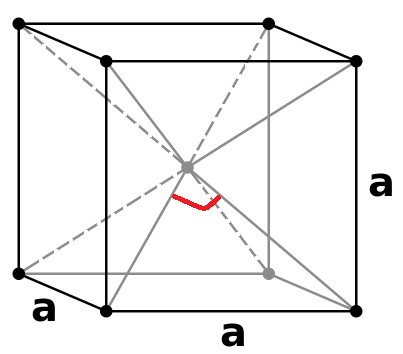
\includegraphics[height = 4cm]{Antoine/Figures_Antoine/BCC2.png}
                \caption{Schéma d'une structure cubique centrée. Les atomes sont matérialisés par les points de jonction du cube. L'atome central se trouve au centre de la structure.}
            \end{figure}
        \end{question}
        \begin{reponses} 
            \item[true] \SI{90}{\degree}
            \item[false] \SI{45}{\degree} 
            \item[false] \SI{180}{\degree}
    	    \item[false] \SI{60}{\degree}
        \end{reponses}
        %%%%%%%%%%%%%%%%%%%%
        \begin{question}{31}{Structure cristalline}{2}{}
            La structure cristalline de l'or est du type \emph{cubique faces centrées} comme montré par le schéma ci-dessous. Quelle est la valeur de l'angle indiqué par un arc de cercle rouge en fonction de $a$, le paramètre de maille? (indice: faites des dessins des différentes vues).
            \begin{figure}
                \centering
                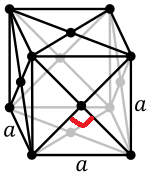
\includegraphics[height = 4cm]{Antoine/Figures_Antoine/FCC2.png}
                \caption{Schéma d'une structure cubique faces centrées. Les atomes sont matérialisés par les points de jonction du cube. Chaque face du cube possède un atome central.}
            \end{figure}
        \end{question}
        \begin{reponses} 
            \item[true] \SI{90}{\degree}
            \item[false] \SI{45}{\degree} 
            \item[false] \SI{180}{\degree}
    	    \item[false] \SI{60}{\degree}
        \end{reponses}
        %%%%%%%%%%%%%%%%%%%%
        \begin{question}{31}{Structures cristallines}{3}{}
            La structure cristalline du niobium est du type \emph{cubique centré} comme montré par le schéma ci-dessous. Si on considère que les atomes sont des boules indéformables collées les unes aux autres de rayon $R$, quelle est l'expression du paramètre de maille $a$ en fonction de $R$? (indice: faites des dessins des différentes vues).
            \begin{figure}
                \centering
                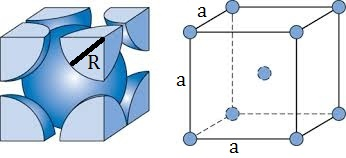
\includegraphics[height = 4cm]{Antoine/Figures_Antoine/BCC.png}
                \caption{Schéma d'une structure cubique centrée. La position des atomes sont matérialisés par les points noirs mais ils se touchent en réalité. L'atome central se trouve au centre de la structure.}
            \end{figure}
        \end{question}
        \begin{reponses} 
            \item[false] $a = 2R$
            \item[false] $a = 4R$
            \item[false] $a = 2R/\sqrt{2}$
    	    \item[true] $a = 4R\sqrt{3}$
        \end{reponses}
        %%%%%%%%%%%%%%%%%%%%
        \begin{question}{31}{Structures cristallines}{3}{}
            La structure cristalline du fer est du type \emph{cubique centré} comme montré par le schéma ci-dessous. Si on considère que les atomes sont des boules indéformables collées les unes aux autres de rayon $R$, quelle est l'expression de la compacité $c = \frac{\text{Volume total de la maille}}{\text{Volume occupé par les atomes}}$ en fonction du paramètre de maille $a$ et/ou de $R$? (indice: faites des dessins des différentes vues. Plusieurs réponses sont possibles).
            \begin{figure}
                \centering
                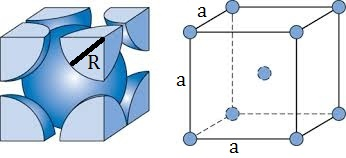
\includegraphics[height = 4cm]{Antoine/Figures_Antoine/BCC.png}
                \caption{Schéma d'une structure cubique centrée. La position des atomes sont matérialisés par les points noirs mais ils se touchent en réalité. L'atome central se trouve au centre de la structure.}
            \end{figure}
        \end{question}
        \begin{reponses} 
            \item[true] $c = \frac{2\times V_\text{atome}}{a^3}$
            \item[false] $c = \frac{9V_\text{atome}}{a^3}$
            \item[true] $c = \frac{8(\pi R^3)}{3a^3}$
    	    \item[false] $c = \frac{3(\pi R^3)}{4a^3}$
        \end{reponses}
        %%%%%%%%%%%%%%%%%%%%
        \begin{question}{31}{Structures cristallines}{3}{}
            La structure cristalline du diamant est du type \emph{cubique faces centrées} comme montré par le schéma ci-dessous. Si on considère que les atomes sont des boules indéformables collées les unes aux autres de rayon $R$, quelle est l'expression du paramètre de maille $a$ en fonction de $R$? (indice: faites des dessins des différentes vues).
            \begin{figure}
                \centering
                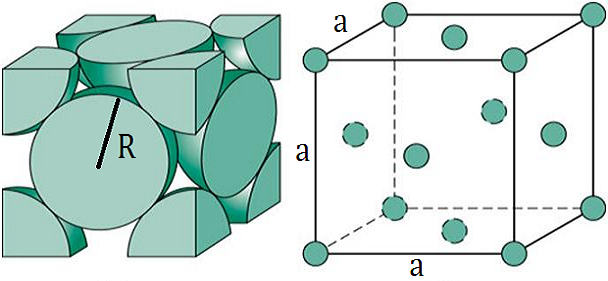
\includegraphics[height = 4cm]{Antoine/Figures_Antoine/FCC.png}
                \caption{Schéma d'une structure cubique faces centrées. La position des atomes sont matérialisés par les points noirs mais ils se touchent en réalité.  Chaque face du cube possède un atome central.}
            \end{figure}
        \end{question}
        \begin{reponses} 
            \item[false] $a = 2R$
            \item[false] $a = 4R$
            \item[false] $a = 2R/\sqrt{3}$
    	    \item[true] $a = 4R\sqrt{2}$
        \end{reponses}
        %%%%%%%%%%%%%%%%%%%%
        \begin{question}{31}{Structures cristallines}{3}{}
            La structure cristalline du silicium est du type \emph{cubique faces centrées} comme montré par le schéma ci-dessous. Si on considère que les atomes sont des boules indéformables collées les unes aux autres de rayon $R$, quelle est l'expression de la compacité $c = \frac{\text{Volume total de la maille}}{\text{Volume occupé par les atomes}}$ en fonction du paramètre de maille $a$ et/ou de $R$? (indice: faites des dessins des différentes vues. Plusieurs réponses sont possibles).
            \begin{figure}
                \centering
                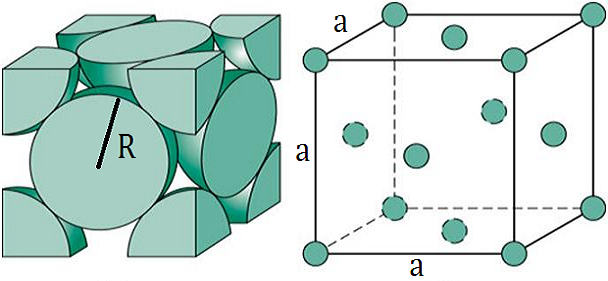
\includegraphics[height = 4cm]{Antoine/Figures_Antoine/FCC.png}
                \caption{Schéma d'une structure cubique faces centrées. La position des atomes sont matérialisés par les points noirs mais ils se touchent en réalité.  Chaque face du cube possède un atome central.}
            \end{figure}
        \end{question}
        \begin{reponses} 
            \item[true] $c = \frac{4\times V_\text{atome}}{a^3}$
            \item[false] $c = \frac{14V_\text{atome}}{a^3}$
            \item[false] $c = \frac{4(\pi R^3)}{3a^3}$
    	    \item[true] $c = \frac{12(\pi R^3)}{4a^3}$
        \end{reponses}
        %%%%%%%%%%%%%%%%%%%%
        \begin{question}{31}{Structures cristallines}{3}{}
            La structure cristalline du silicium est du type \emph{cubique faces centrées} comme montré par le schéma ci-dessous. Si on considère que les atomes sont des boules indéformables collées les unes aux autres de rayon $R$. La compacité $c = \frac{\text{Volume total de la maille}}{\text{Volume occupé par les atomes}}$, renseigne sur l'espace libre disponible dans un cristal. Connaître $c$ est utile pour doper le cristal avec d'autres éléments, ce qui est très utile en physique des semi-conducteurs où l'ajout d'autres éléments à un cristal change ses propriétés électriques. Quelle est la valeur de ce paramètre pour cette maille? (indice: faites des dessins des différentes vues).
            \begin{figure}
                \centering
                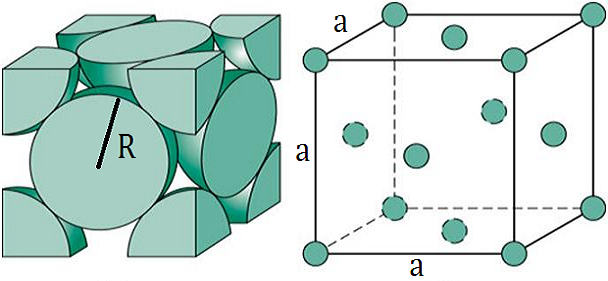
\includegraphics[height = 4cm]{Antoine/Figures_Antoine/FCC.png}
                \caption{Schéma d'une structure cubique faces centrées. La position des atomes sont matérialisés par les points noirs mais ils se touchent en réalité.  Chaque face du cube possède un atome central.}
            \end{figure}
        \end{question}
        \begin{reponses} 
            \item[true] $c = \frac{\pi\sqrt{2}}{6}$
            \item[false] $c = 12$
            \item[false] $c = \frac{3\sqrt{2}}{5}$
    	    \item[false] $c = \num{0.5}$
        \end{reponses}
        %%%%%%%%%%%%%%%%%%%%
        \begin{question}{31}{Structures cristallines}{3}{}
            La structure cristalline du fer est du type \emph{cubique centré} comme montré par le schéma ci-dessous. Si on considère que les atomes sont des boules indéformables collées les unes aux autres de rayon $R$. La compacité $c = \frac{\text{Volume total de la maille}}{\text{Volume occupé par les atomes}}$, renseigne sur l'espace libre disponible dans un cristal. Connaître $c$ est utile pour doper le cristal avec d'autres éléments, ce qui est très utile en physique des semi-conducteurs où l'ajout d'autres éléments à un cristal change ses propriétés électriques. Quelle est la valeur de ce paramètre pour cette maille? (indice: faites des dessins des différentes vues).
            \begin{figure}
                \centering
                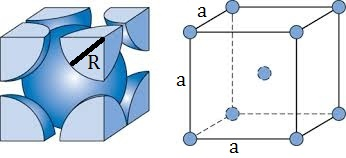
\includegraphics[height = 4cm]{Antoine/Figures_Antoine/BCC.png}
                \caption{Schéma d'une structure cubique centrée. La position des atomes sont matérialisés par les points noirs mais ils se touchent en réalité. L'atome central se trouve au centre de la structure.}
            \end{figure}
        \end{question}
        \begin{reponses} 
            \item[true] $c = \frac{\pi\sqrt{3}}{8}$
            \item[false] $c = \frac{\pi\sqrt{3}}{4}$
            \item[false] $c = \frac{\pi\sqrt{2}}{8}$
    	    \item[false] $c = \num{.5}$
        \end{reponses}
        %%%%%%%%%%%%%%%%%%%%
